\documentclass[tikz,border=22pt]{standalone}
\usepackage[T1]{fontenc}
\usepackage{helvet}
\renewcommand{\familydefault}{\sfdefault}
\usepackage{amsmath,amssymb}
\usetikzlibrary{calc,positioning,fit,backgrounds,shapes.geometric,shapes.symbols,arrows.meta,decorations.pathreplacing}

% =============================================================================
% CANONICAL MLSYSBOOK PALETTE
% =============================================================================
\definecolor{DarkSlate}{HTML}{0F172A}
\definecolor{slatesteel}{HTML}{334155}
\definecolor{BlueLine}{HTML}{006395}
\definecolor{BlueL}{RGB}{209,243,255}
\definecolor{BlueL0}{HTML}{F0F9FF}
\definecolor{GreenLine}{HTML}{008F45}
\definecolor{GreenL}{RGB}{219,253,166}
\definecolor{GreenL0}{HTML}{EBF8F2}
\definecolor{forestsage}{HTML}{166534}
\definecolor{OrangeLine}{HTML}{E67817}
\definecolor{OrangeL}{RGB}{254,237,222}
\definecolor{OrangeL0}{HTML}{FFFBEB}
\definecolor{warmochre}{HTML}{92400E}
\definecolor{RedLine}{HTML}{D9534F}
\definecolor{RedL}{RGB}{253,226,240}
\definecolor{RedL0}{HTML}{FEF2F2}
\definecolor{deepburgundy}{HTML}{991B1B}
\definecolor{VioletLine}{HTML}{7E317B}
\definecolor{VioletL}{RGB}{247,215,247}
\definecolor{amethyst}{HTML}{581C87}
\definecolor{amethystL0}{HTML}{FAF5FF}
\definecolor{GrayLine}{HTML}{64748B}
\definecolor{coolparchment}{HTML}{F8FAFC}
\definecolor{CardBorder}{HTML}{CBD5E1}
\definecolor{ChipBlack}{HTML}{181F2C}
\definecolor{GoldPin}{HTML}{EAB308}

\tikzset{
  >=Latex,
  font=\sffamily,
  flow_arrow/.style={->, >=Latex, line width=1.1pt},
  flow_arrow_thick/.style={->, >=Latex, line width=1.5pt},
}

\begin{document}
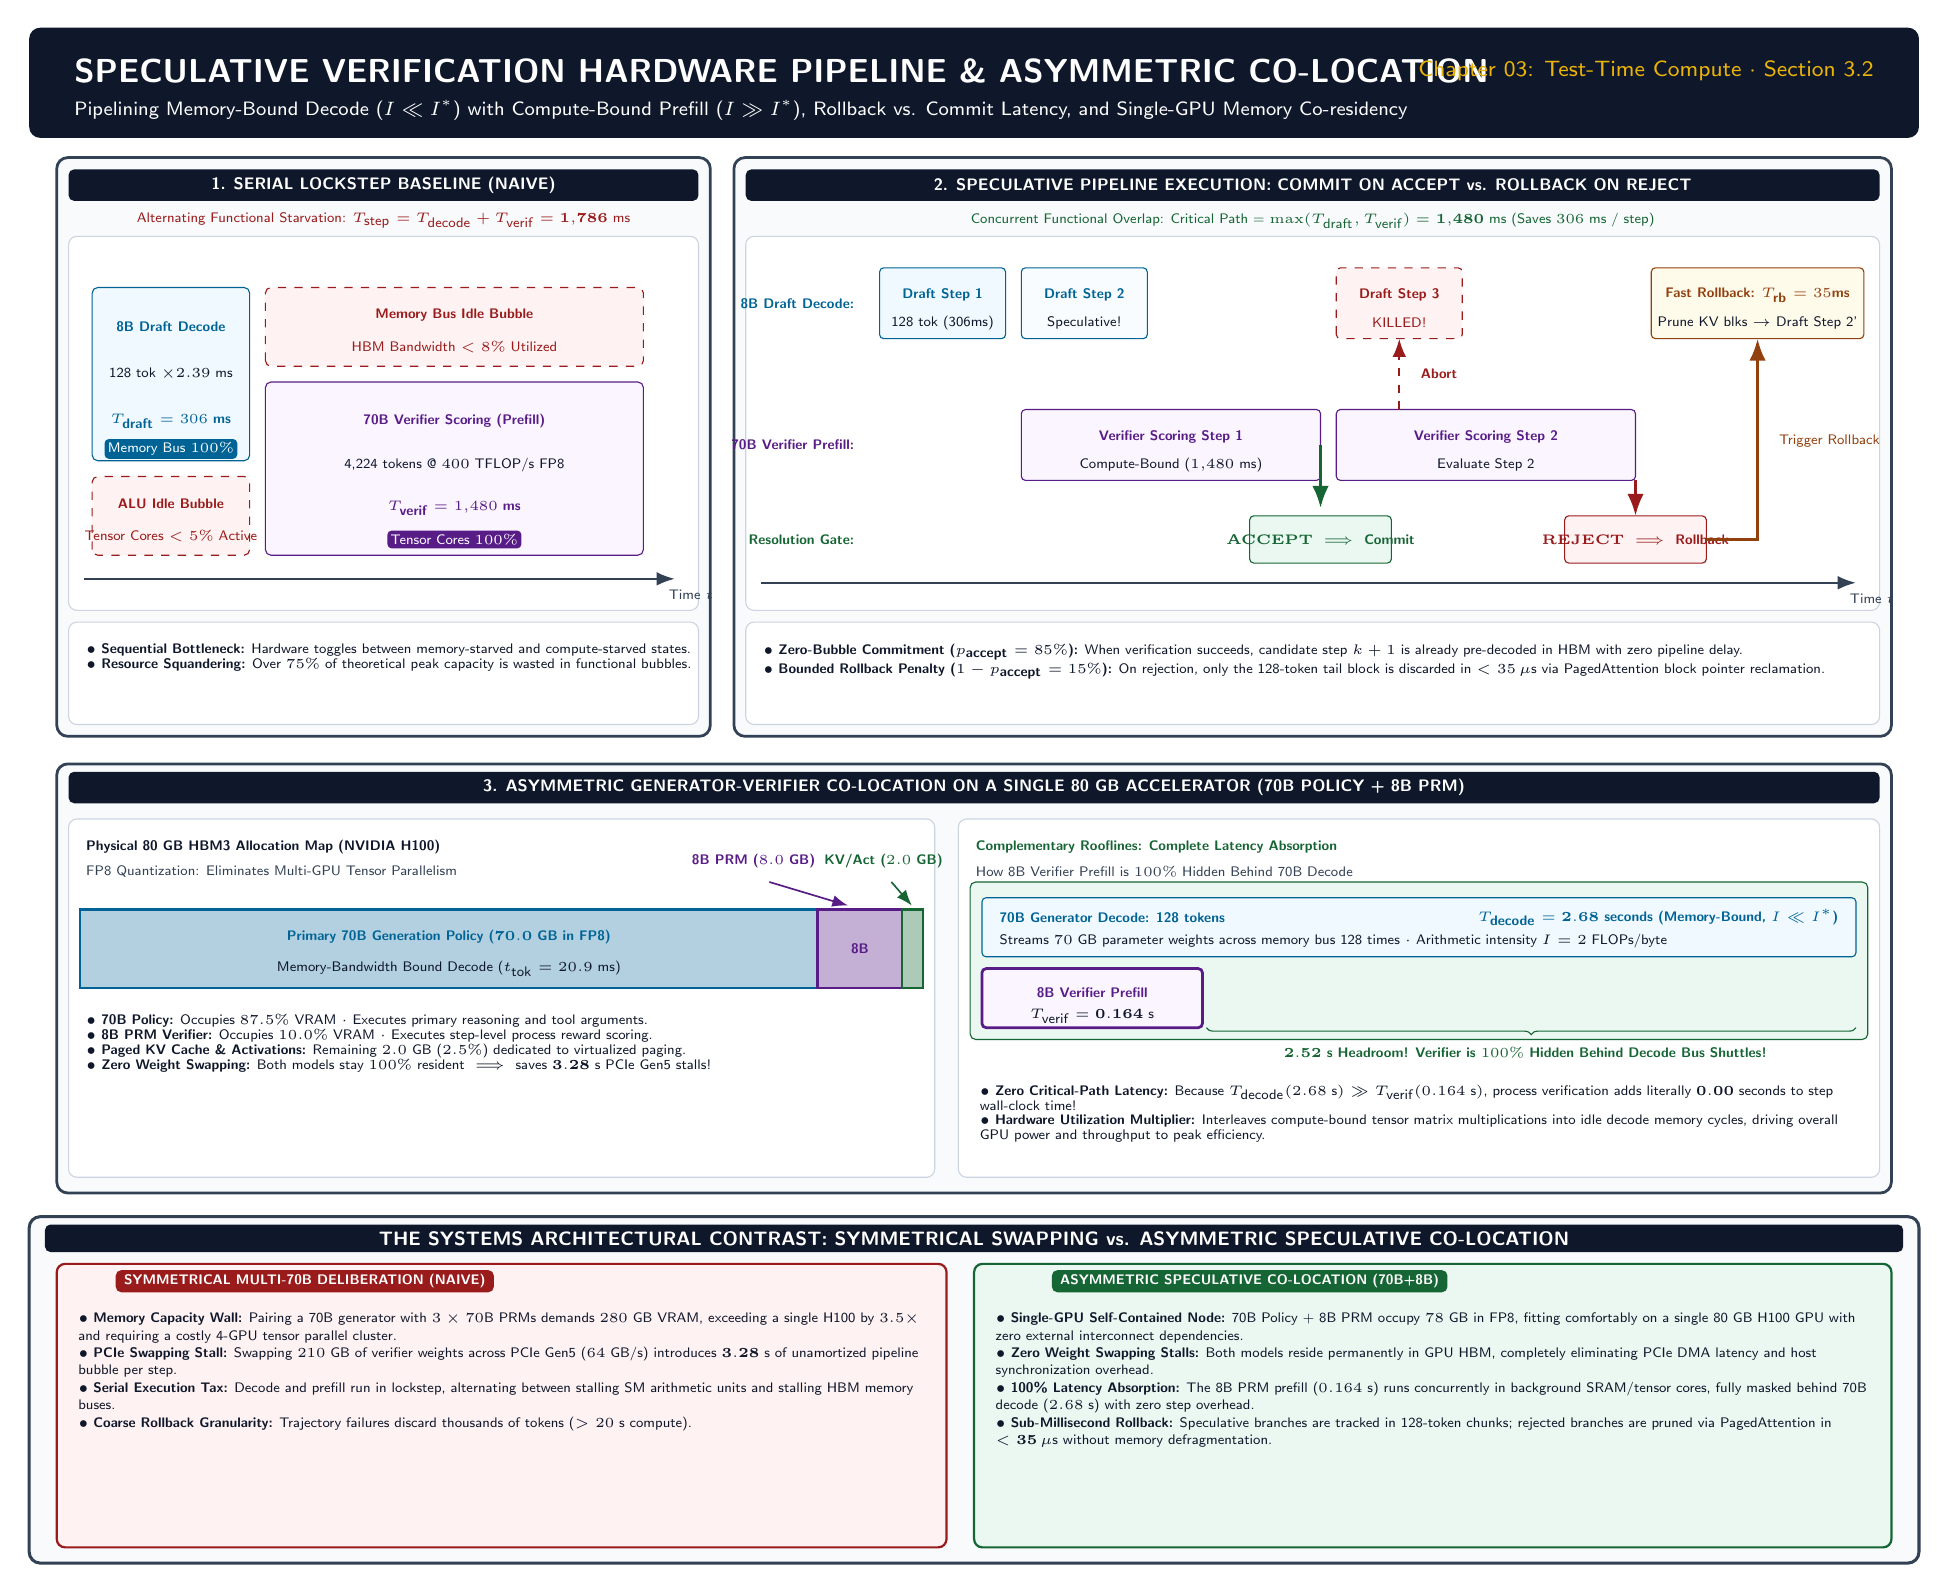
\begin{tikzpicture}[x=1cm, y=1cm]

% =============================================================================
% TOP TITLE BANNER (y: 18.6 to 20.0)
% =============================================================================
\draw[fill=DarkSlate, draw=none, rounded corners=4pt] (0, 18.6) rectangle (24.0, 20.0);
\node[anchor=west, font=\bfseries\large, text=white] at (0.45, 19.45) {
  SPECULATIVE VERIFICATION HARDWARE PIPELINE \& ASYMMETRIC CO-LOCATION
};
\node[anchor=east, font=\footnotesize, text=GoldPin] at (23.55, 19.45) {
  Chapter 03: Test-Time Compute $\cdot$ Section 3.2
};
\node[anchor=west, font=\scriptsize, text=white!85] at (0.45, 18.95) {
  Pipelining Memory-Bound Decode ($I \ll I^*$) with Compute-Bound Prefill ($I \gg I^*$), Rollback vs. Commit Latency, and Single-GPU Memory Co-residency
};

% =============================================================================
% TIER 1: HARDWARE EXECUTION TIMELINE: SERIAL LOCKSTEP vs. SPECULATIVE PIPELINE (y: 11.00 to 18.35)
% =============================================================================

% --- Left Panel: Serial Lockstep Baseline (x: 0.35 to 8.65) ---
\draw[draw=slatesteel, fill=coolparchment, line width=1.0pt, rounded corners=4pt] (0.35, 11.00) rectangle (8.65, 18.35);

\fill[DarkSlate, rounded corners=2pt] (0.5, 17.80) rectangle (8.5, 18.20);
\node[font=\bfseries\fontsize{5.8pt}{6.8pt}\selectfont, text=white] at (4.50, 18.00) {
  1. SERIAL LOCKSTEP BASELINE (NAIVE)
};

% Subtitle
\node[font=\fontsize{4.6pt}{5.6pt}\selectfont, text=deepburgundy] at (4.50, 17.55) {
  Alternating Functional Starvation: $T_{\text{step}} = T_{\text{decode}} + T_{\text{verif}} = \mathbf{1{,}786\text{ ms}}$
};

% Timeline Graphic for Serial (y: 12.60 to 17.20)
\draw[draw=CardBorder, fill=white, rounded corners=3pt] (0.5, 12.60) rectangle (8.5, 17.35);

% Axis
\draw[->, line width=0.8pt, draw=slatesteel] (0.7, 13.00) -- (8.2, 13.00);
\node[anchor=west, font=\fontsize{4.2pt}{5.2pt}\selectfont, text=slatesteel] at (8.0, 12.80) {Time $t$};

% Step 1: Draft Decode (8B, 306 ms)
\draw[draw=BlueLine, fill=BlueL0, rounded corners=2pt] (0.8, 14.50) rectangle (2.8, 16.70);
\node[font=\bfseries\fontsize{5.0pt}{6.0pt}\selectfont, text=BlueLine] at (1.8, 16.20) {8B Draft Decode};
\node[font=\fontsize{4.4pt}{5.4pt}\selectfont, text=DarkSlate] at (1.8, 15.60) {128 tok $\times 2.39\text{ ms}$};
\node[font=\bfseries\fontsize{5.0pt}{6.0pt}\selectfont, text=BlueLine] at (1.8, 15.00) {$T_{\text{draft}} = 306\text{ ms}$};
\node[draw=none, fill=BlueLine, rounded corners=1.5pt, text=white, font=\fontsize{3.8pt}{4.8pt}\selectfont, inner sep=1.2pt] at (1.8, 14.65) {Memory Bus $100\%$};

% Bubble 1: ALU Idle Bubble (during Draft Decode)
\draw[draw=deepburgundy, fill=RedL0, rounded corners=2pt, dashed] (0.8, 13.30) rectangle (2.8, 14.30);
\node[font=\bfseries\fontsize{4.4pt}{5.4pt}\selectfont, text=deepburgundy] at (1.8, 13.95) {ALU Idle Bubble};
\node[font=\fontsize{4.0pt}{5.0pt}\selectfont, text=deepburgundy] at (1.8, 13.55) {Tensor Cores $< 5\%$ Active};

% Step 2: 70B Verifier Prefill (1,480 ms)
\draw[draw=amethyst, fill=amethystL0, rounded corners=2pt] (3.0, 13.30) rectangle (7.8, 15.50);
\node[font=\bfseries\fontsize{5.0pt}{6.0pt}\selectfont, text=amethyst] at (5.4, 15.00) {70B Verifier Scoring (Prefill)};
\node[font=\fontsize{4.4pt}{5.4pt}\selectfont, text=DarkSlate] at (5.4, 14.45) {4,224 tokens @ $400\text{ TFLOP/s}$ FP8};
\node[font=\bfseries\fontsize{5.0pt}{6.0pt}\selectfont, text=amethyst] at (5.4, 13.90) {$T_{\text{verif}} = 1{,}480\text{ ms}$};
\node[draw=none, fill=amethyst, rounded corners=1.5pt, text=white, font=\fontsize{3.8pt}{4.8pt}\selectfont, inner sep=1.2pt] at (5.4, 13.50) {Tensor Cores $100\%$};

% Bubble 2: Bus Idle Bubble (during Verifier Prefill)
\draw[draw=deepburgundy, fill=RedL0, rounded corners=2pt, dashed] (3.0, 15.70) rectangle (7.8, 16.70);
\node[font=\bfseries\fontsize{4.4pt}{5.4pt}\selectfont, text=deepburgundy] at (5.4, 16.35) {Memory Bus Idle Bubble};
\node[font=\fontsize{4.0pt}{5.0pt}\selectfont, text=deepburgundy] at (5.4, 15.95) {HBM Bandwidth $< 8\%$ Utilized};

% Bottom Summary Box for Serial
\draw[draw=CardBorder, fill=white, rounded corners=3pt] (0.5, 11.15) rectangle (8.5, 12.45);
\node[anchor=north west, font=\fontsize{4.5pt}{5.5pt}\selectfont, text=DarkSlate] at (0.6, 12.30) {
  \begin{minipage}{7.8cm}\raggedright
    $\bullet$ \textbf{Sequential Bottleneck:} Hardware toggles between memory-starved and compute-starved states.\\
    $\bullet$ \textbf{Resource Squandering:} Over $75\%$ of theoretical peak capacity is wasted in functional bubbles.
  \end{minipage}
};

% --- Right Panel: Speculative Verification Pipeline (x: 8.95 to 23.65) ---
\draw[draw=slatesteel, fill=coolparchment, line width=1.0pt, rounded corners=4pt] (8.95, 11.00) rectangle (23.65, 18.35);

\fill[DarkSlate, rounded corners=2pt] (9.1, 17.80) rectangle (23.5, 18.20);
\node[font=\bfseries\fontsize{5.8pt}{6.8pt}\selectfont, text=white] at (16.30, 18.00) {
  2. SPECULATIVE PIPELINE EXECUTION: COMMIT ON ACCEPT vs. ROLLBACK ON REJECT
};

\node[font=\fontsize{4.6pt}{5.6pt}\selectfont, text=forestsage] at (16.30, 17.55) {
  Concurrent Functional Overlap: Critical Path = $\max(T_{\text{draft}}, T_{\text{verif}}) = \mathbf{1{,}480\text{ ms}}$ (Saves $306\text{ ms}$ / step)
};

% Timeline Graphic for Pipelined (y: 12.60 to 17.35)
\draw[draw=CardBorder, fill=white, rounded corners=3pt] (9.1, 12.60) rectangle (23.5, 17.35);

% Axis
\draw[->, line width=0.8pt, draw=slatesteel] (9.3, 12.95) -- (23.2, 12.95);
\node[anchor=west, font=\fontsize{4.2pt}{5.2pt}\selectfont, text=slatesteel] at (23.0, 12.75) {Time $t$};

% Row Labels
\node[anchor=east, font=\bfseries\fontsize{4.4pt}{5.4pt}\selectfont, text=BlueLine] at (10.6, 16.50) {8B Draft Decode:};
\node[anchor=east, font=\bfseries\fontsize{4.4pt}{5.4pt}\selectfont, text=amethyst] at (10.6, 14.70) {70B Verifier Prefill:};
\node[anchor=east, font=\bfseries\fontsize{4.4pt}{5.4pt}\selectfont, text=forestsage] at (10.6, 13.50) {Resolution Gate:};

% --- Turn 1: Commit Flow (x: 10.8 to 16.6) ---
% Step 1 Draft
\draw[draw=BlueLine, fill=BlueL0, rounded corners=1.5pt] (10.8, 16.05) rectangle (12.4, 16.95);
\node[font=\bfseries\fontsize{4.4pt}{5.4pt}\selectfont, text=BlueLine] at (11.6, 16.60) {Draft Step 1};
\node[font=\fontsize{3.8pt}{4.8pt}\selectfont, text=DarkSlate] at (11.6, 16.25) {128 tok (306ms)};

% Step 2 Draft (Speculative!)
\draw[draw=BlueLine, fill=BlueL0!50, rounded corners=1.5pt] (12.6, 16.05) rectangle (14.2, 16.95);
\node[font=\bfseries\fontsize{4.4pt}{5.4pt}\selectfont, text=BlueLine] at (13.4, 16.60) {Draft Step 2};
\node[font=\fontsize{3.8pt}{4.8pt}\selectfont, text=DarkSlate] at (13.4, 16.25) {Speculative!};

% Step 1 Verifier Prefill (Running concurrently with Step 2 Draft!)
\draw[draw=amethyst, fill=amethystL0, rounded corners=1.5pt] (12.6, 14.25) rectangle (16.4, 15.15);
\node[font=\bfseries\fontsize{4.4pt}{5.4pt}\selectfont, text=amethyst] at (14.5, 14.80) {Verifier Scoring Step 1};
\node[font=\fontsize{3.8pt}{4.8pt}\selectfont, text=DarkSlate] at (14.5, 14.45) {Compute-Bound ($1{,}480\text{ ms}$)};

% Verifier Decision Arrow & Gate
\draw[flow_arrow, draw=forestsage] (16.4, 14.70) -- (16.4, 13.90);
\draw[draw=forestsage, fill=GreenL0, rounded corners=1.5pt] (15.5, 13.20) rectangle (17.3, 13.80);
\node[font=\bfseries\fontsize{4.4pt}{5.4pt}\selectfont, text=forestsage] at (16.4, 13.50) {$\mathbf{ACCEPT}$ $\implies$ \textbf{Commit}};

% --- Turn 2: Rollback Flow (x: 17.5 to 23.3) ---
% Step 3 Draft (Speculative!)
\draw[draw=deepburgundy, fill=RedL0, rounded corners=1.5pt, dashed] (16.6, 16.05) rectangle (18.2, 16.95);
\node[font=\bfseries\fontsize{4.4pt}{5.4pt}\selectfont, text=deepburgundy] at (17.4, 16.60) {Draft Step 3};
\node[font=\fontsize{3.8pt}{4.8pt}\selectfont, text=deepburgundy] at (17.4, 16.25) {KILLED!};

% Step 2 Verifier Prefill
\draw[draw=amethyst, fill=amethystL0, rounded corners=1.5pt] (16.6, 14.25) rectangle (20.4, 15.15);
\node[font=\bfseries\fontsize{4.4pt}{5.4pt}\selectfont, text=amethyst] at (18.5, 14.80) {Verifier Scoring Step 2};
\node[font=\fontsize{3.8pt}{4.8pt}\selectfont, text=DarkSlate] at (18.5, 14.45) {Evaluate Step 2};

% Verifier Decision Rejection Gate
\draw[flow_arrow, draw=deepburgundy] (20.4, 14.25) -- (20.4, 13.80);
\draw[draw=deepburgundy, fill=RedL0, rounded corners=1.5pt] (19.5, 13.20) rectangle (21.3, 13.80);
\node[font=\bfseries\fontsize{4.4pt}{5.4pt}\selectfont, text=deepburgundy] at (20.4, 13.50) {$\mathbf{REJECT}$ $\implies$ \textbf{Rollback}};

% Flow Arrows from Reject:
% 1) Abort speculative draft (clean vertical arrow directly into Draft Step 3)
\draw[->, draw=deepburgundy, dashed, line width=0.8pt] (17.4, 15.15) -- (17.4, 16.05);
\node[anchor=west, font=\bfseries\fontsize{3.8pt}{4.8pt}\selectfont, text=deepburgundy] at (17.55, 15.60) {Abort};

% 2) Trigger fast rollback (clean orthogonal line)
\draw[flow_arrow, draw=warmochre] (21.3, 13.50) -| (21.95, 16.05);
\node[anchor=west, font=\fontsize{4.0pt}{5.0pt}\selectfont, text=warmochre] at (22.10, 14.75) {Trigger Rollback};

% Rollback Recovery Block
\draw[draw=warmochre, fill=OrangeL0, rounded corners=1.5pt] (20.6, 16.05) rectangle (23.3, 16.95);
\node[font=\bfseries\fontsize{4.2pt}{5.2pt}\selectfont, text=warmochre] at (21.95, 16.60) {Fast Rollback: $T_{\text{rb}} = 35\text{ms}$};
\node[font=\fontsize{3.8pt}{4.8pt}\selectfont, text=DarkSlate] at (21.95, 16.25) {Prune KV blks $\to$ Draft Step 2'};

% Connecting curly brace on Step 1
\draw[decorate, decoration={brace, amplitude=3pt, mirror}, draw=slatesteel] (10.8, 12.45) -- (16.4, 12.45);
\node[font=\fontsize{4.2pt}{5.2pt}\selectfont, text=slatesteel] at (13.6, 12.15) {Pipelined Step 1 Latency: $1{,}480\text{ ms}$ (Saves $306\text{ ms}$)};

% Bottom Summary Box for Pipelined
\draw[draw=CardBorder, fill=white, rounded corners=3pt] (9.1, 11.15) rectangle (23.5, 12.45);
\node[anchor=north west, font=\fontsize{4.5pt}{5.5pt}\selectfont, text=DarkSlate] at (9.2, 12.30) {
  \begin{minipage}{14.1cm}\raggedright
    $\bullet$ \textbf{Zero-Bubble Commitment ($p_{\text{accept}} = 85\%$):} When verification succeeds, candidate step $k+1$ is already pre-decoded in HBM with zero pipeline delay.\\
    $\bullet$ \textbf{Bounded Rollback Penalty ($1 - p_{\text{accept}} = 15\%$):} On rejection, only the 128-token tail block is discarded in $<35\,\mu\text{s}$ via PagedAttention block pointer reclamation.
  \end{minipage}
};

% =============================================================================
% TIER 2: ASYMMETRIC GENERATOR-VERIFIER CO-LOCATION (y: 5.20 to 10.65)
% =============================================================================
\draw[draw=slatesteel, fill=coolparchment, line width=1.0pt, rounded corners=4pt] (0.35, 5.20) rectangle (23.65, 10.65);

\fill[DarkSlate, rounded corners=2pt] (0.5, 10.15) rectangle (23.5, 10.55);
\node[font=\bfseries\fontsize{6.2pt}{7.2pt}\selectfont, text=white] at (12.00, 10.35) {
  3. ASYMMETRIC GENERATOR-VERIFIER CO-LOCATION ON A SINGLE 80 GB ACCELERATOR (70B POLICY + 8B PRM)
};

% Left Box: Physical VRAM Map (x: 0.5 to 11.5, y: 5.40 to 9.95)
\draw[draw=CardBorder, fill=white, rounded corners=3pt] (0.5, 5.40) rectangle (11.5, 9.95);
\node[anchor=north west, font=\bfseries\fontsize{5.2pt}{6.2pt}\selectfont, text=DarkSlate] at (0.6, 9.80) {Physical 80 GB HBM3 Allocation Map (NVIDIA H100)};
\node[anchor=north west, font=\fontsize{4.4pt}{5.4pt}\selectfont, text=slatesteel] at (0.6, 9.48) {FP8 Quantization: Eliminates Multi-GPU Tensor Parallelism};

% Memory Bar (Horizontal Stack)
\draw[draw=slatesteel, line width=0.8pt] (0.65, 7.80) rectangle (11.35, 8.80);

% 70B Policy Segment (70 GB = 87.5% of bar)
\fill[BlueLine!30] (0.65, 7.80) rectangle (10.01, 8.80);
\draw[draw=BlueLine, line width=0.8pt] (0.65, 7.80) rectangle (10.01, 8.80);
\node[font=\bfseries\fontsize{5.0pt}{6.0pt}\selectfont, text=BlueLine] at (5.33, 8.45) {Primary 70B Generation Policy ($\mathbf{70.0\text{ GB}}$ in FP8)};
\node[font=\fontsize{4.4pt}{5.4pt}\selectfont, text=DarkSlate] at (5.33, 8.05) {Memory-Bandwidth Bound Decode ($t_{\text{tok}} = 20.9\text{ ms}$)};

% 8B PRM Segment (8 GB = 10.0% of bar)
\fill[amethyst!35] (10.01, 7.80) rectangle (11.08, 8.80);
\draw[draw=amethyst, line width=0.8pt] (10.01, 7.80) rectangle (11.08, 8.80);
\node[font=\bfseries\fontsize{4.4pt}{5.4pt}\selectfont, text=amethyst] at (10.55, 8.30) {8B};

% Activation + KV (2 GB = 2.5% of bar)
\fill[forestsage!35] (11.08, 7.80) rectangle (11.35, 8.80);
\draw[draw=forestsage, line width=0.8pt] (11.08, 7.80) rectangle (11.35, 8.80);

% Non-overlapping callouts above the bar (strictly within x in [0.5, 11.5]):
% 8B PRM Callout (centered at x = 9.2, pointing to 10.55)
\node[anchor=south, font=\bfseries\fontsize{4.2pt}{5.2pt}\selectfont, text=amethyst] at (9.20, 9.20) {8B PRM ($8.0\text{ GB}$)};
\draw[->, line width=0.6pt, amethyst] (9.40, 9.15) -- (10.40, 8.85);

% KV/Act Callout (centered at x = 10.85, pointing to 11.21, width fits safely before 11.45)
\node[anchor=south, font=\bfseries\fontsize{4.2pt}{5.2pt}\selectfont, text=forestsage] at (10.85, 9.20) {KV/Act ($2.0\text{ GB}$)};
\draw[->, line width=0.6pt, forestsage] (10.95, 9.15) -- (11.21, 8.85);

% Legend below bar
\node[anchor=north west, font=\fontsize{4.5pt}{5.5pt}\selectfont, text=DarkSlate] at (0.6, 7.60) {
  \begin{minipage}{10.7cm}\raggedright
    $\bullet$ \textbf{70B Policy:} Occupies $87.5\%$ VRAM $\cdot$ Executes primary reasoning and tool arguments.\\
    $\bullet$ \textbf{8B PRM Verifier:} Occupies $10.0\%$ VRAM $\cdot$ Executes step-level process reward scoring.\\
    $\bullet$ \textbf{Paged KV Cache \& Activations:} Remaining $2.0\text{ GB}$ ($2.5\%$) dedicated to virtualized paging.\\
    $\bullet$ \textbf{Zero Weight Swapping:} Both models stay $100\%$ resident $\implies$ saves $\mathbf{3.28\text{ s}}$ PCIe Gen5 stalls!
  \end{minipage}
};

% Right Box: Roofline Complementarity & Latency Absorption (x: 11.8 to 23.5, y: 5.40 to 9.95)
\draw[draw=CardBorder, fill=white, rounded corners=3pt] (11.8, 5.40) rectangle (23.5, 9.95);
\node[anchor=north west, font=\bfseries\fontsize{5.2pt}{6.2pt}\selectfont, text=forestsage] at (11.9, 9.80) {Complementary Rooflines: Complete Latency Absorption};
\node[anchor=north west, font=\fontsize{4.4pt}{5.4pt}\selectfont, text=slatesteel] at (11.9, 9.48) {How 8B Verifier Prefill is $100\%$ Hidden Behind 70B Decode};

% Absorption Timeline Box
\draw[draw=forestsage, fill=GreenL0, rounded corners=2pt] (11.95, 7.15) rectangle (23.35, 9.15);

% 70B Generator Decode Bar (Long, 2.68s)
\draw[draw=BlueLine, fill=BlueL0, rounded corners=1.5pt] (12.1, 8.20) rectangle (23.2, 8.95);
\node[anchor=west, font=\bfseries\fontsize{4.6pt}{5.6pt}\selectfont, text=BlueLine] at (12.2, 8.70) {70B Generator Decode: 128 tokens};
\node[anchor=east, font=\bfseries\fontsize{4.6pt}{5.6pt}\selectfont, text=BlueLine] at (23.1, 8.70) {$T_{\text{decode}} = \mathbf{2.68\text{ seconds}}$ (Memory-Bound, $I \ll I^*$)};
\node[anchor=west, font=\fontsize{4.0pt}{5.0pt}\selectfont, text=DarkSlate] at (12.2, 8.40) {Streams $70\text{ GB}$ parameter weights across memory bus 128 times $\cdot$ Arithmetic intensity $I = 2\text{ FLOPs/byte}$};

% 8B Verifier Burst (Short, 0.164s, perfectly absorbed inside!)
\draw[draw=amethyst, fill=amethystL0, line width=1.0pt, rounded corners=1.5pt] (12.1, 7.30) rectangle (14.9, 8.05);
\node[font=\bfseries\fontsize{4.4pt}{5.4pt}\selectfont, text=amethyst] at (13.5, 7.75) {8B Verifier Prefill};
\node[font=\fontsize{3.8pt}{4.8pt}\selectfont, text=DarkSlate] at (13.5, 7.45) {$T_{\text{verif}} = \mathbf{0.164\text{ s}}$};

% Bracket & Absorption Note
\draw[decorate, decoration={brace, amplitude=2.5pt, mirror}, draw=forestsage] (14.95, 7.30) -- (23.2, 7.30);
\node[anchor=north, font=\bfseries\fontsize{4.4pt}{5.4pt}\selectfont, text=forestsage] at (19.0, 7.18) {
  $\mathbf{2.52\text{ s}}$ Headroom! Verifier is $100\%$ Hidden Behind Decode Bus Shuttles!
};

\node[anchor=north west, font=\fontsize{4.4pt}{5.4pt}\selectfont, text=DarkSlate] at (11.95, 6.70) {
  \begin{minipage}{11.2cm}\raggedright
    $\bullet$ \textbf{Zero Critical-Path Latency:} Because $T_{\text{decode}} (2.68\text{ s}) \gg T_{\text{verif}} (0.164\text{ s})$, process verification adds literally $\mathbf{0.00\text{ seconds}}$ to step wall-clock time!\\
    $\bullet$ \textbf{Hardware Utilization Multiplier:} Interleaves compute-bound tensor matrix multiplications into idle decode memory cycles, driving overall GPU power and throughput to peak efficiency.
  \end{minipage}
};

% =============================================================================
% TIER 3: SYSTEMS ARCHITECTURAL CONTRAST (y: 0.50 to 4.90)
% =============================================================================
\draw[draw=slatesteel, fill=coolparchment, line width=1.1pt, rounded corners=4pt] (0, 0.50) rectangle (24.0, 4.90);

\fill[DarkSlate, rounded corners=2pt] (0.2, 4.45) rectangle (23.8, 4.80);
\node[font=\bfseries\fontsize{6.8pt}{8.2pt}\selectfont, text=white] at (12.0, 4.62) {
  THE SYSTEMS ARCHITECTURAL CONTRAST: SYMMETRICAL SWAPPING vs. ASYMMETRIC SPECULATIVE CO-LOCATION
};

% Left Box: Symmetrical Multi-GPU Swapping (x: 0.35 to 11.65)
\draw[draw=deepburgundy, fill=RedL0, rounded corners=3pt, line width=0.8pt] (0.35, 0.70) rectangle (11.65, 4.30);
\node[draw=none, fill=deepburgundy, rounded corners=2pt, inner xsep=3pt, inner ysep=1.5pt, font=\bfseries\fontsize{5.5pt}{6.5pt}\selectfont, text=white] at (3.5, 4.08) {
  SYMMETRICAL MULTI-70B DELIBERATION (NAIVE)
};

\node[anchor=north west, font=\fontsize{5.0pt}{6.3pt}\selectfont, text=DarkSlate] at (0.5, 3.80) {
  \begin{minipage}{10.8cm}\raggedright
    $\bullet$ \textbf{Memory Capacity Wall:} Pairing a 70B generator with $3 \times 70\text{B}$ PRMs demands $280\text{ GB}$ VRAM, exceeding a single H100 by $3.5\times$ and requiring a costly 4-GPU tensor parallel cluster.\\
    $\bullet$ \textbf{PCIe Swapping Stall:} Swapping $210\text{ GB}$ of verifier weights across PCIe Gen5 ($64\text{ GB/s}$) introduces $\mathbf{3.28\text{ s}}$ of unamortized pipeline bubble per step.\\
    $\bullet$ \textbf{Serial Execution Tax:} Decode and prefill run in lockstep, alternating between stalling SM arithmetic units and stalling HBM memory buses.\\
    $\bullet$ \textbf{Coarse Rollback Granularity:} Trajectory failures discard thousands of tokens ($>20\text{ s}$ compute).
  \end{minipage}
};

% Right Box: Speculative Asymmetric Co-Location (x: 12.00 to 23.65)
\draw[draw=forestsage, fill=GreenL0, rounded corners=3pt, line width=0.8pt] (12.0, 0.70) rectangle (23.65, 4.30);
\node[draw=none, fill=forestsage, rounded corners=2pt, inner xsep=3pt, inner ysep=1.5pt, font=\bfseries\fontsize{5.5pt}{6.5pt}\selectfont, text=white] at (15.5, 4.08) {
  ASYMMETRIC SPECULATIVE CO-LOCATION (70B+8B)
};

\node[anchor=north west, font=\fontsize{5.0pt}{6.3pt}\selectfont, text=DarkSlate] at (12.15, 3.80) {
  \begin{minipage}{11.1cm}\raggedright
    $\bullet$ \textbf{Single-GPU Self-Contained Node:} 70B Policy + 8B PRM occupy $78\text{ GB}$ in FP8, fitting comfortably on a single 80 GB H100 GPU with zero external interconnect dependencies.\\
    $\bullet$ \textbf{Zero Weight Swapping Stalls:} Both models reside permanently in GPU HBM, completely eliminating PCIe DMA latency and host synchronization overhead.\\
    $\bullet$ \textbf{100\% Latency Absorption:} The 8B PRM prefill ($0.164\text{ s}$) runs concurrently in background SRAM/tensor cores, fully masked behind 70B decode ($2.68\text{ s}$) with zero step overhead.\\
    $\bullet$ \textbf{Sub-Millisecond Rollback:} Speculative branches are tracked in 128-token chunks; rejected branches are pruned via PagedAttention in $<\mathbf{35\,\mu\text{s}}$ without memory defragmentation.
  \end{minipage}
};

\end{tikzpicture}
\end{document}
